%%% PREAMBLE %%%

% Strict mode

\RequirePackage[l2tabu, orthodox]{nag} % Warn when using deprecated constructs

% Document class and packages

\documentclass[10pt,a4paper,parskip,fleqn]{scrartcl}
\usepackage[a4paper,vmargin={22mm},hmargin={30mm}]{geometry} % Page margins
\usepackage[ngerman]{babel} % New German hyphenation (multilingual support)
\usepackage[utf8x]{inputenc} % Unicode support
\usepackage{graphicx} % Graphics support
\usepackage{enumitem} % List spacing
\usepackage{nopageno} % No page numbers
\usepackage{chngpage} % Adjust page width
\usepackage{calc} % Calculations
\usepackage{color} % Colors
\usepackage[colorlinks=true, urlcolor=black]{hyperref} % Hyperlinks
\usepackage{subfig} % Subfigures (für fotos)
\usepackage{float} % H placing specifier

\captionsetup[figure]{font=small,aboveskip=4pt,belowskip=8pt}

% Font configuration

\usepackage[sc]{mathpazo} % Use palatino font
\usepackage[T1]{fontenc} % Use correct font encoding
\usepackage[babel=true]{microtype} % Micro-typographic optimizations
\usepackage{setspace} % Line spacing
\addtokomafont{disposition}{\rmfamily} % Set palatino as heading font
\setstretch{1.3}
\setlist{nolistsep} % No spacing in lists

% Constants

\newcommand{\membercount}{26}


%%% TITLEPAGE %%%

\title{\Huge Coredump Rapperswil}
\subject{Sponsoring-Anfrage}


%%% MAIN DOCUMENT %%%

\begin{document}

\begin{titlepage}

	\maketitle

	\vspace{2cm}

	\begin{adjustwidth}{-\oddsidemargin-1in}{-\rightmargin-1in}
		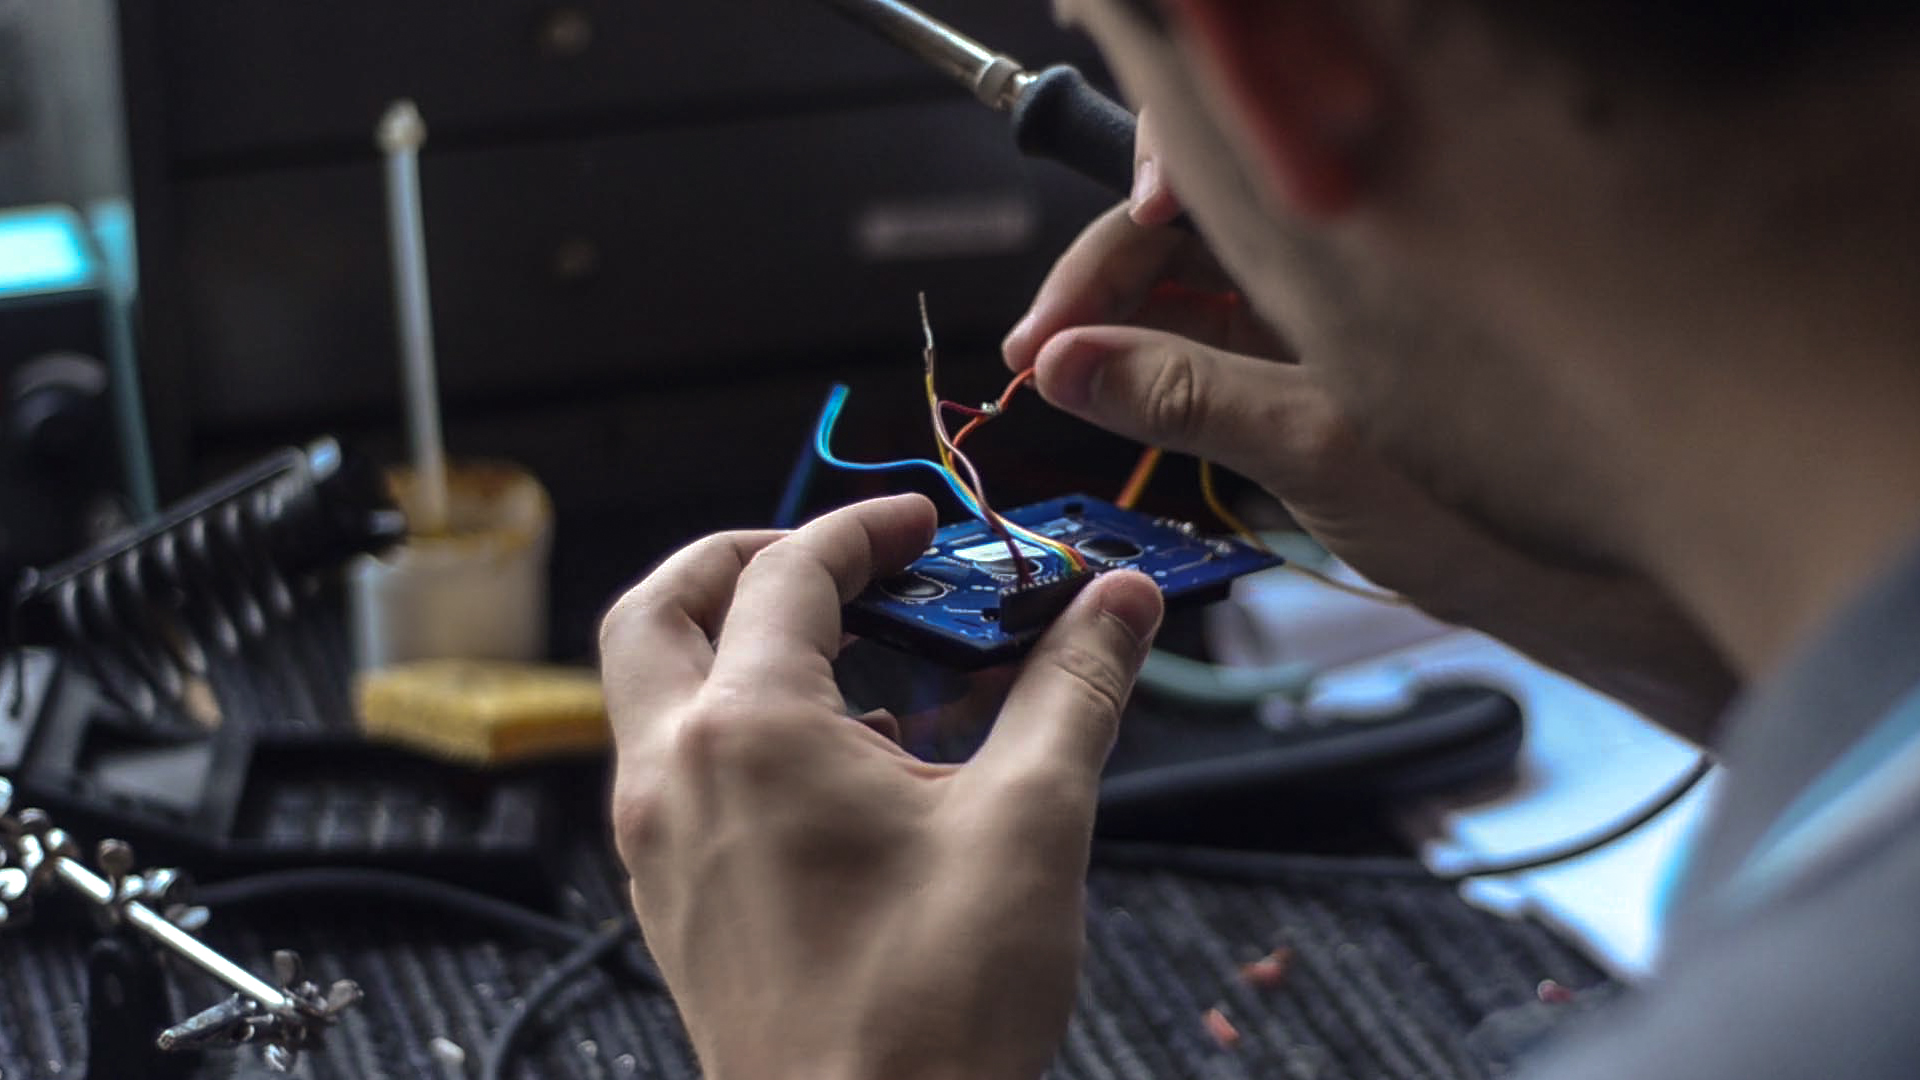
\includegraphics[width=\paperwidth]{img/soldering.jpg}

		\vspace{-12mm}

		\definecolor{light-gray}{gray}{0.85}
		\hfill {\scriptsize \color{light-gray} CC BY-NC-SA flickr.com/cbeas}
	\end{adjustwidth}

	\vfill

\end{titlepage}

\section{Management Summary}

Auf dieser Seite finden Sie eine stichwortartige Zusammenfassung des gesamten
Dokumentes.

\subsection{Über Uns}

\begin{itemize}
	\item Wir sind ein Verein, welcher Technikbegeisterten in Rapperswil und
		Umgebung die technische Infrastruktur für nichtkommerzielle Projekte
		anbietet. Daneben verfolgen wir auch Bildungsprojekte wie Kurse im Rahmen
		des Ferienpass Rapperswil-Jona oder öffentliche Vorträge.
	\item Unser Vereinsraum bietet Platz zum Arbeiten, eine Elektronik-Werkstatt mit
		Lötstationen und Messgeräten, einen 3D-Drucker, eine kleine Bibliothek, eine
		Sitzecke mit Getränkekühlschrank und vieles mehr.
	\item Unser 100m²-Vereinsraum befindet sich auf dem Vinora-Areal in
		Rapperswil-Jona.
	\item Aktuell haben wir \membercount{} Aktivmitglieder.
	\item Unser typisches Mitglied ist zwischen 25 und 30 Jahre alt, wobei wir
		auch jüngere und ältere Mitglieder haben. Viele der Mitglieder haben ein
		Elektrotechnik- oder Informatikstudium hinter sich oder studieren aktuell
		noch.
	\item Besucher sind jederzeit willkommen. Wir treffen uns jeden Montag ab 20
		Uhr.
	\item Einige Projekte unserer Mitglieder: Low-power Wassertemperatursensoren
		für den Obersee mit LoRaWAN, farbige interaktive LED-Steuerungen für
		Outdoor-Festivals, orthopädische Alltagshilfen aus dem 3D-Drucker, selber
		entwickelte Open Source PCB-Design-Software, eine selbst gebaute
		Tesla-Spule, ein mithilfe von Drohnen erfasstes 3D-Modell des Schloss
		Rapperswils, eine selbstgebaute Infrarot-Fernbedienung für
		Canon-Spiegelreflexkameras und vieles mehr.
\end{itemize}

\subsection{Finanzierung}

\begin{itemize}
	\item Wir finanzieren uns primär über die Mitgliederbeiträge und private
		Gönner. Ein Nichtverdienermitglied bezahlt 10 CHF pro Monat, ein
		Verdienermitglied 30 CHF pro Monat und ein Fördermitglied 50 CHF pro Monat.
	\item Obwohl unser Verein stetig wächst, benötigen wir momentan noch weitere
		finanzielle Unterstützung von Sponsoren oder Gönnern -- primär zur Deckung
		der Fixkosten und zum Verbessern unserer Einrichtung und Ausrüstung.
	\item Als Gegenleistung erhält der Sponsor einen Werbeplatz in unserem
		Vereinsraum. Darauf könnten Sie beispielsweise Ihre Firma vorstellen oder
		Jobangebote publizieren.
	\item Desweiteren erhält der Sponsor einen stets sichtbaren Link oder ein Logo
		auf unserer Website (\href{https://www.coredump.ch/}{\texttt{coredump.ch}})
		und wird in einem öffentlichen Blogpost sowie an jeder GV den Mitgliedern
		vorgestellt.
	\item Sponsoring-Pakete: Small (80 CHF im Monat), Medium (120 CHF im Monat)
		oder Large (180 CHF im Monat). Andere Beträge sind nach Absprache auch
		möglich.
\end{itemize}

Weitere Informationen finden Sie auf den folgenden Seiten sowie auf
\href{https://www.coredump.ch/}{\texttt{coredump.ch}}.

\newpage

\section{Über Uns}

Als erster Hackerspace\footnote{Mehr Informationen dazu gibt es auf
\url{http://hackerspaces.org/}} in der Region Linth-Obersee bieten wir Computer-
und Technikbegeisterten seit August 2013 eine Plattform, in der sie ihr Wissen
weitergeben, sich austauschen und Neues lernen können. Damit reihen wir uns in
eine weltweite Bewegung von tausenden von Hackerspaces, Makerspaces, FabLabs,
Techniklabors und ähnlichen Vereinen ein. Unser Angebot ist in der Region des
oberen Zürichsees bisher einzigartig.

Es geht dabei nicht um das kriminelle <<Hacken von Computern>>, wie es in den
Medien häufig dargestellt wird, sondern gemäss der ursprünglichen Definition
eines Hackers\footnote{Mehr zur ursprünglichen Definition eines Hackers gibt es
auf Wikipedia: \url{https://de.wikipedia.org/wiki/Hacker}} um den kreativen
Umgang mit Technik und Wissen. Wir bieten Infrastruktur und Know-How, um
nichtkommerzielle Projekte alleine oder in Kollaboration zu realisieren.

Unser geräumiger 100m²-Vereinsraum auf dem Vinora-Areal in Jona bietet aktuell
eine Elektronikwerkstatt mit Lötstationen, Reflow-Ofen, Labornetzteilen,
Mikroskop und Messgeräten, einen 3D-Drucker mit diversen Druckmaterialien, eine
PCB-Fräse sowie eine Ätz-Station mit UV-Belichtungsgerät zum Herstellen von
PCBs, Arbeitsplätze für mitgebrachte Laptops, WLAN mit Internetverbindung, ein
Lager mit Elektronikbauteilen und Entwicklungs-Kits, eine kleine Bibliothek mit
Fachliteratur, zwei Kühlschränke und eine Mikrowelle für die Verpflegung vor
Ort.

In unserem Hackerspace möchten wir einerseits die Möglichkeiten und das Umfeld
zur Umsetzung von interessanten technischen oder künstlerischen Projekten
anbieten, andererseits aber auch den Austausch von Wissen fördern. Dies kann
regelmässige Treffen, öffentliche Kurzvorträge oder auch Bildungsangebote und
Workshops für interessierte Aussenstehende (z.B. Ferienpass-Kurse für
Schulkinder) beinhalten.

\begin{figure}[h!]
	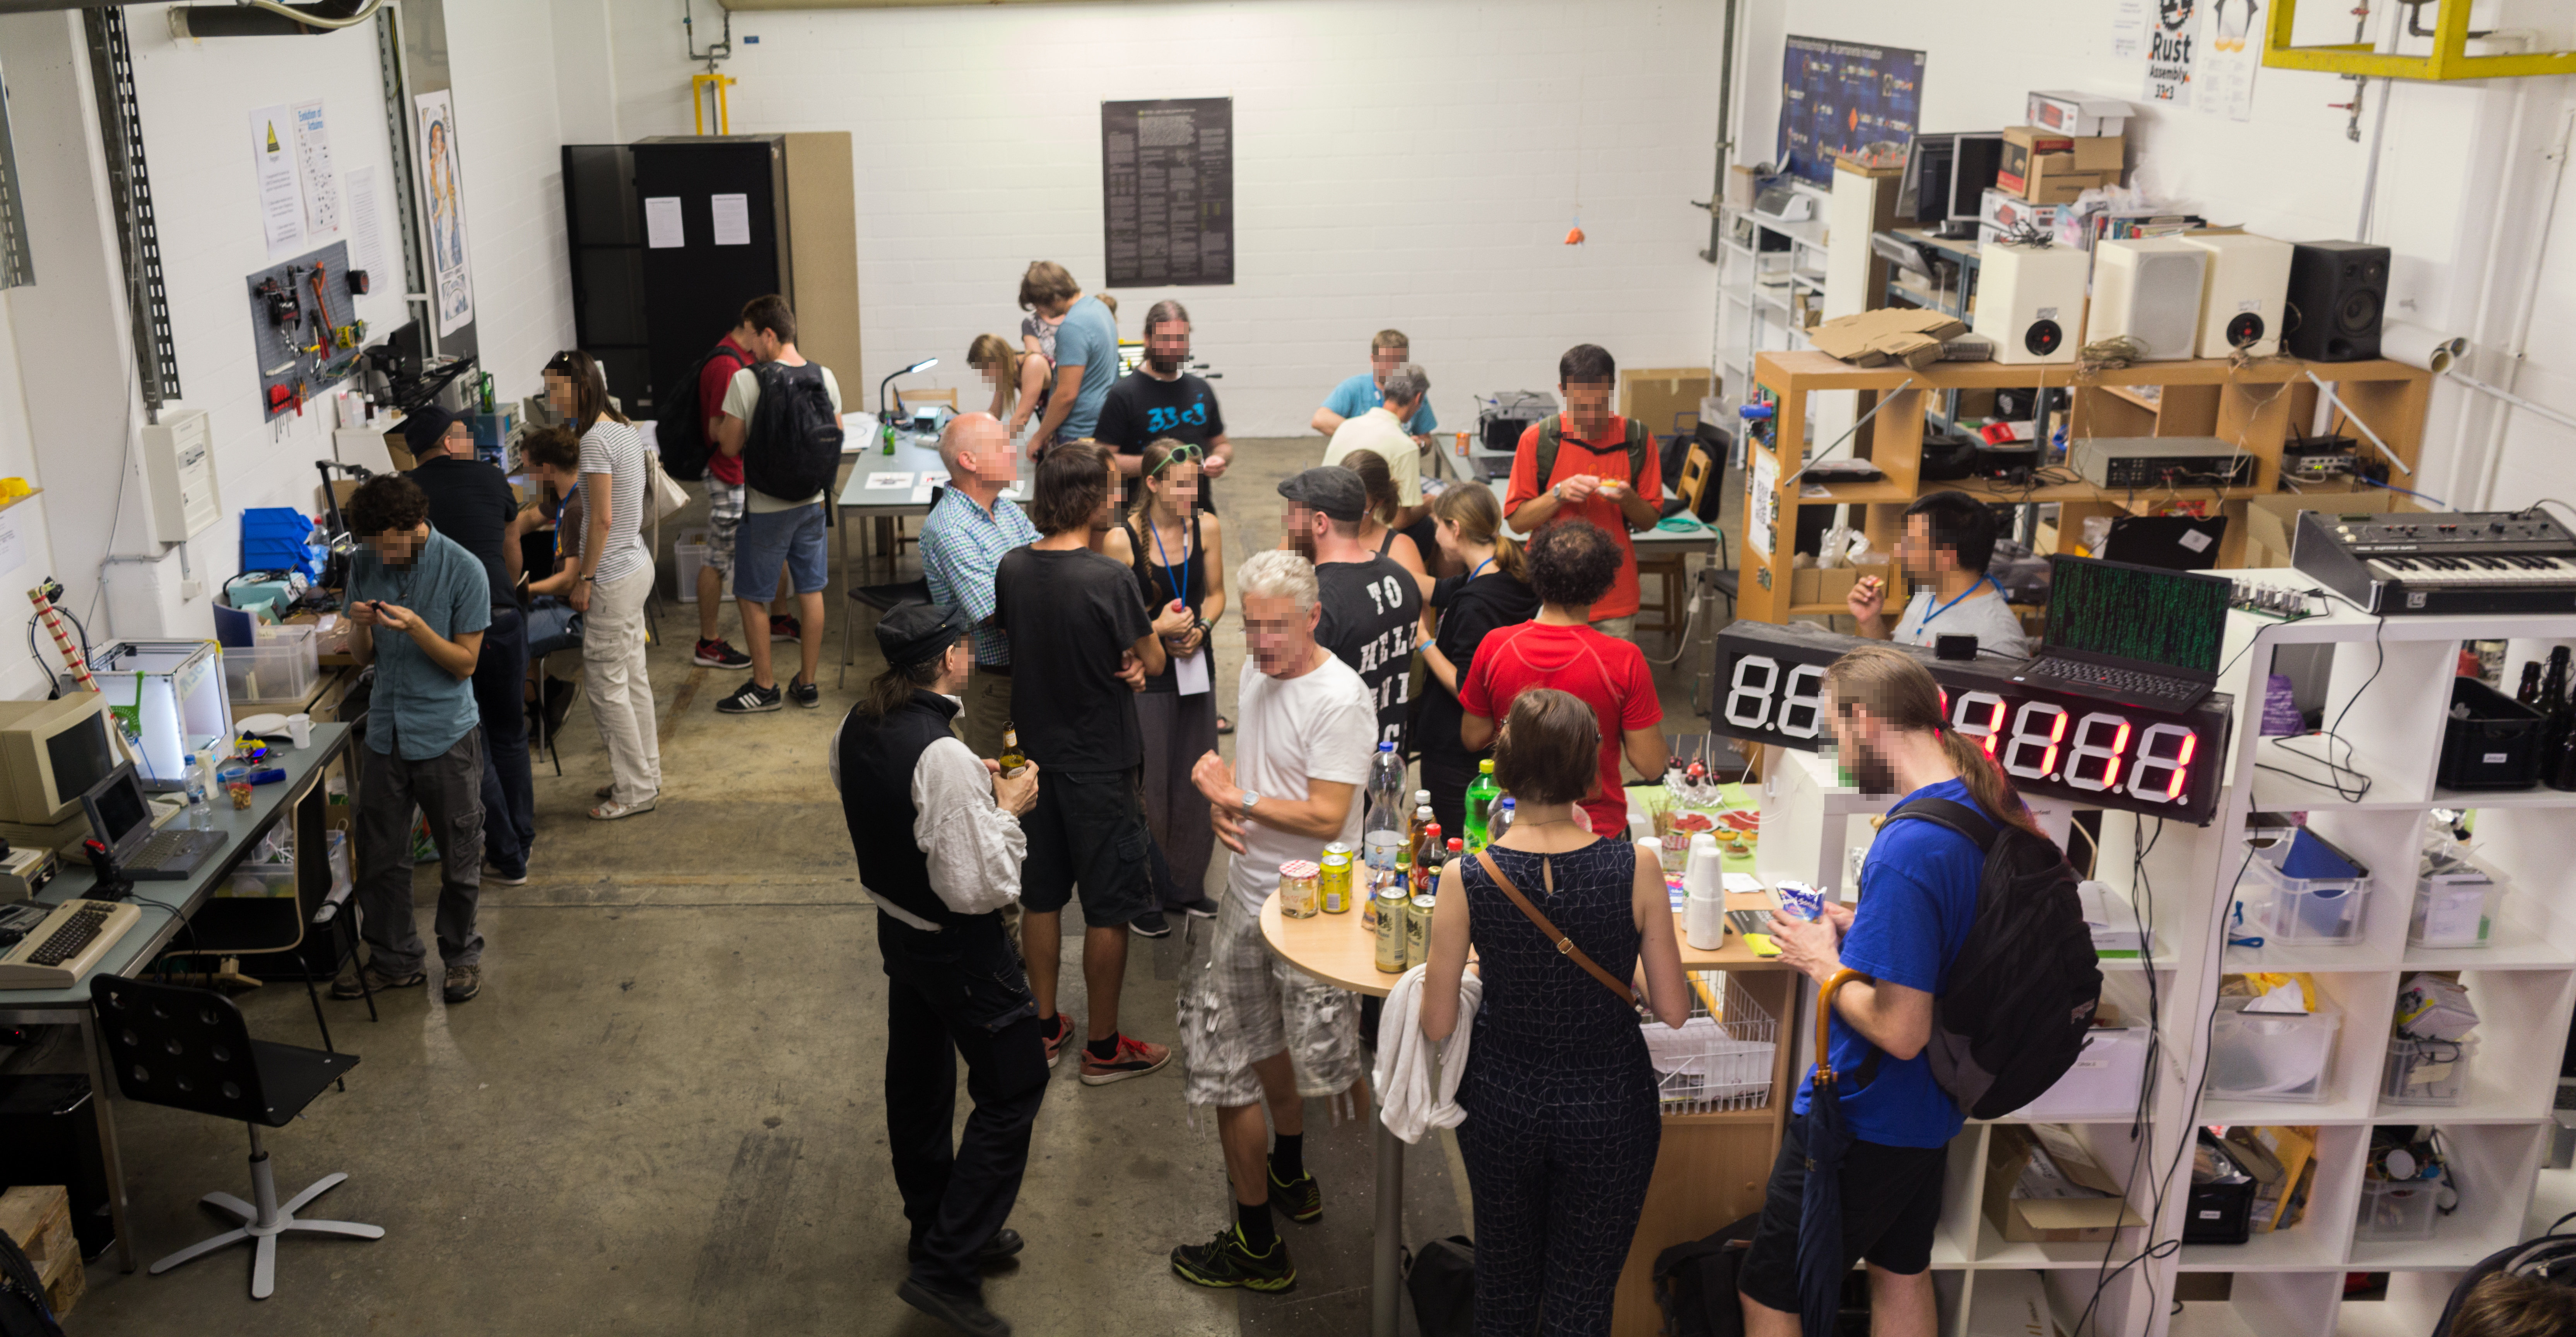
\includegraphics[width=\textwidth]{img/eroeffnungsfest.jpg}
	\caption{Eröffnungsfest Vinora-Areal im August 2018}
\end{figure}

\section{Projekte}

Damit Sie sich ein Bild unserer Aktivitäten machen können, vier unserer
aktuellen Projekte:

\textbf{Gfrör.li: Wassertemperatursensoren Zürichsee}

Derzeit ist es für badefreudige Personen am Obersee schwierig, herauszufinden
wie warm oder kalt der See aktuell ist. Wir möchten deshalb in Kooperation mit
lokalen Vereinen sowie der Hochschule für Technik HSR den Obersee (und später
den Rest des Zürichsees) mit einem Netzwerk aus Wassertemperatur-Sensoren mit
LoRaWAN-Funktechnik ausstatten und diese Messdaten öffentlich über Mobile Apps
sowie auch über Programmier-Schnittstellen zugänglich machen. Den aktuellen
Prototypen finden Sie unter
\texttt{\href{https://xn--gfrr-7qa.li/}{https://gfrör.li/}}.

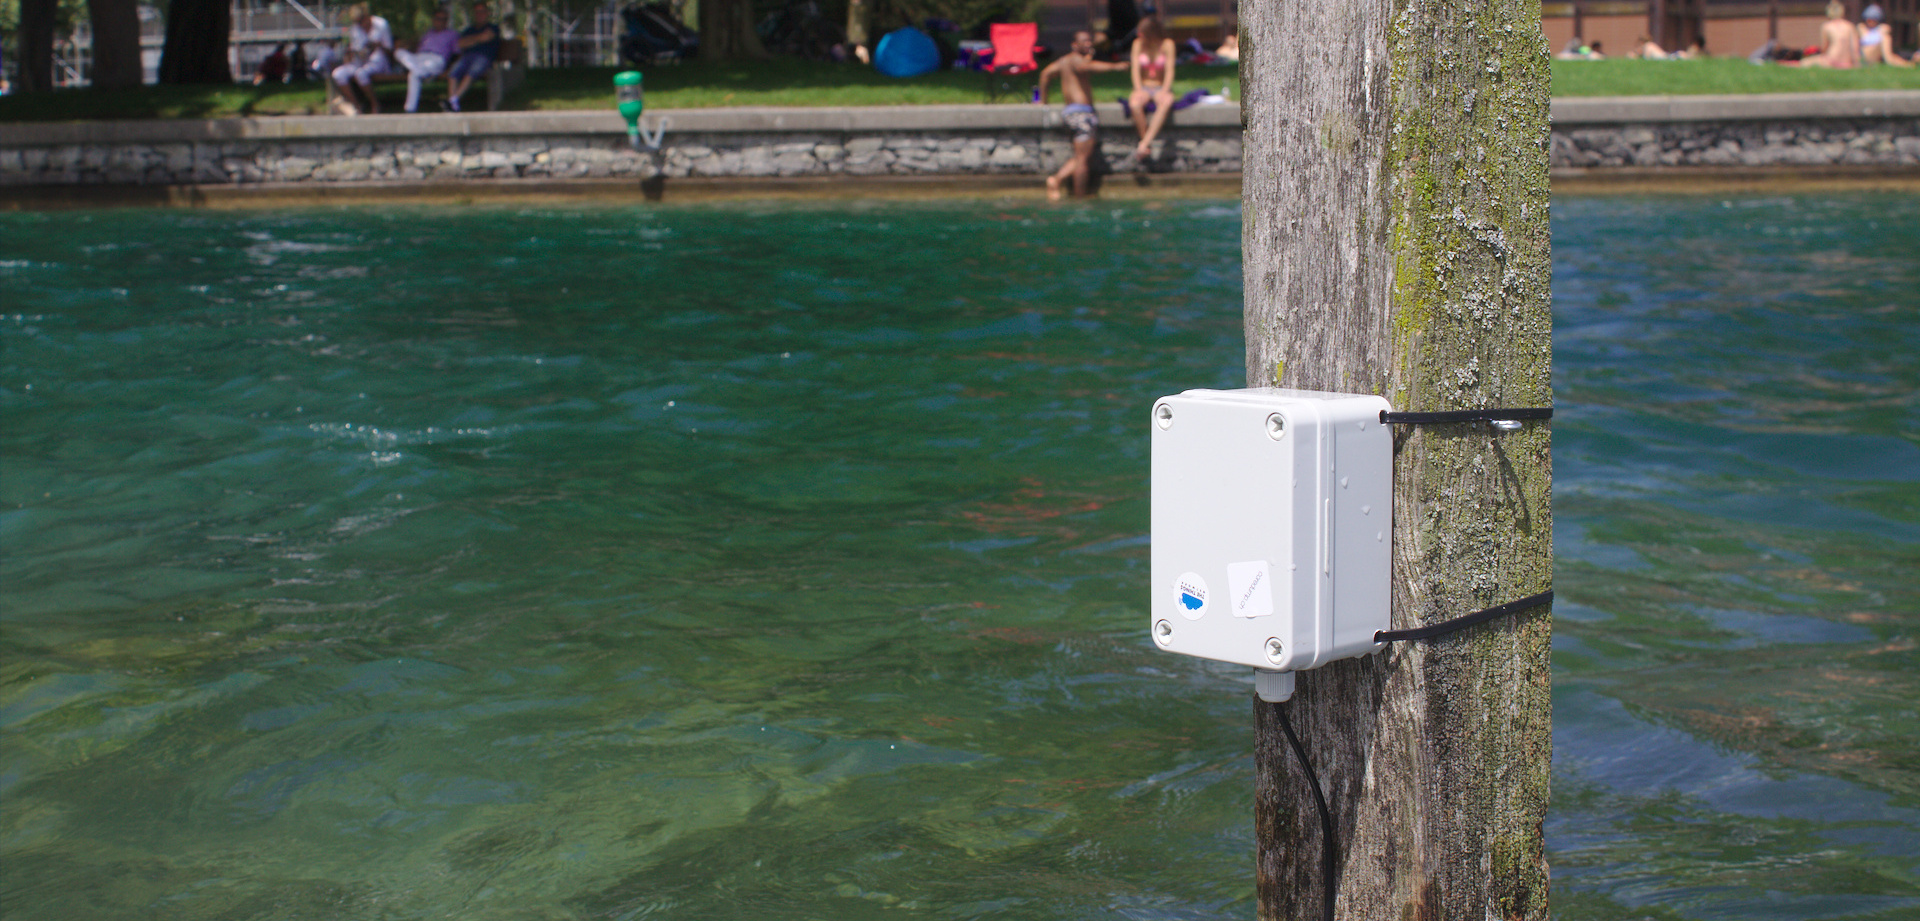
\includegraphics[width=\textwidth]{img/gfroerli.jpg}

\textbf{Ferienpass im Computer- und Technikbereich}

Im November 2014 boten wir zum ersten Mal im Rahmen des Ferienpasses
Rapperswil-Jona einen Löt- und einen Programmierkurs für Kinder an. Diese -- wie
auch wir -- waren davon begeistert: Wir erhielten 86 Anmeldungen und
konnten davon aus Platzgründen leider nur 16 berücksichtigen. Auch im Herbst
2015, 2016 und 2018 boten wir wieder FePa-Kurse an, mit sehr positivem
Feedback. Wir freuen uns darauf, auch in Zukunft weiterhin Schulkinder aus
Rapperswil-Jona für Technik zu begeistern.

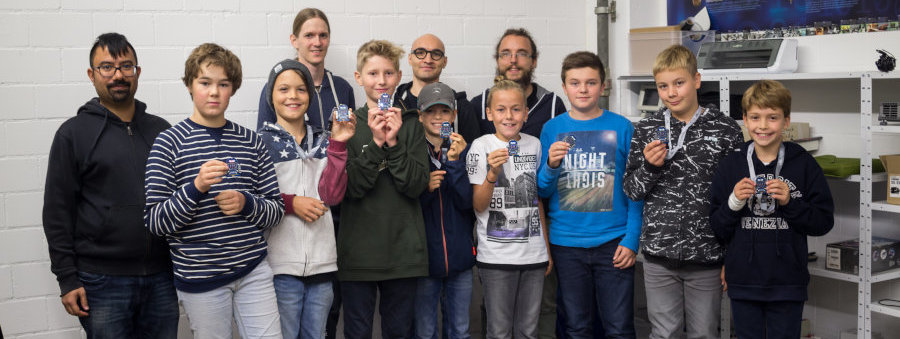
\includegraphics[width=\textwidth]{img/fepa3.jpg}

\textbf{3D-Druck}

Im Jahr 2015 durften wir unseren ersten 3D-Drucker in Betrieb nehmen,
erfolgreich finanziert über die Schweizer Crowdfunding-Plattform ``Wemakeit''.
Im Rahmen dieser Aktion haben wir unter anderem mit Hilfe eines Quadrokopters
einen 3D-Scan des Schlosses Rapperswil erstellt, diese Daten in Kooperation mit
der Hochschule für Technik HSR sowie dem Rapperswiler Start-Up ``Drei-De''
aufbereitet und ein druckfertiges Modell erzeugt.

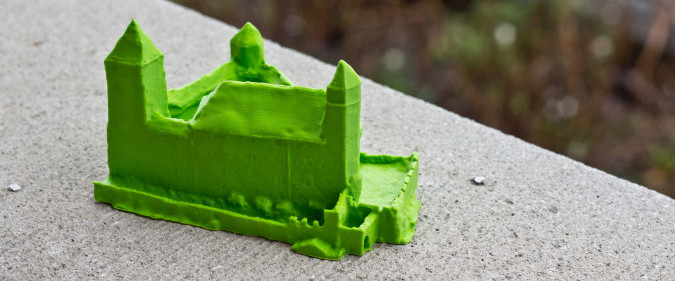
\includegraphics[width=\textwidth]{img/schloss-slim.jpg}

\textbf{LibrePCB}

Eines unserer Mitglieder arbeitet seit vielen Jahren an der Open Source
EDA-Software LibrePCB, welche kostenlos genutzt werden kann um elektronische
Schaltungen und Leiterplatten zu entwerfen, bis hin zu fertigen
Produktionsdaten. Die Version 0.1 wurde im November 2018 veröffentlicht. Weitere
Informationen finden sich unter \url{https://librepcb.org/}.

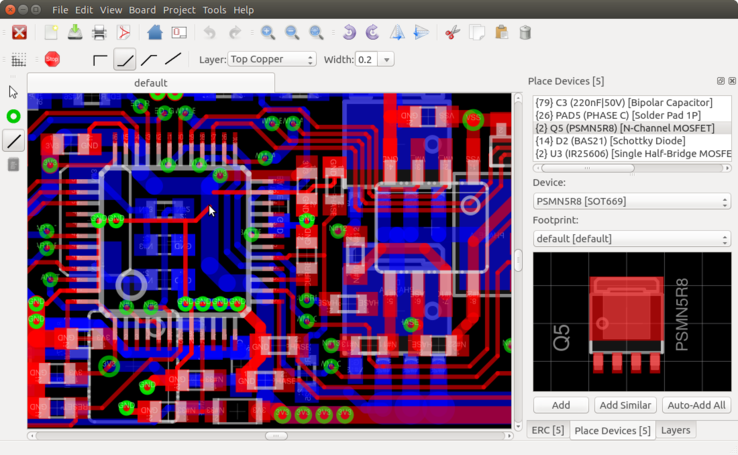
\includegraphics[width=\textwidth]{img/librepcb.png}

\section{Finanzierung}

Bisher finanzieren wir uns primär über die Mitgliederbeiträge. Ein
Nichtverdiener-Mitglied bezahlt bei uns 10~CHF im Monat, ein Verdiener-Mitglied
30~CHF und ein Fördermitglied 50~CHF. Aktuell beläuft sich unsere
Mitglieder-Anzahl auf \membercount{} Personen, die meisten davon sind entweder
Studenten an der HSR oder haben bereits eine technische Ausbildung hinter sich.
Daneben haben wir einige private Gönner.

Unser Verein wächst stetig. Im Jahr 2016 sind wir aus Platzmangel aus unserem
ersten 16m²-Vereinsraum in neue Räumlichkeiten im Sonnenhof umgezogen, gefolgt
von einem weiteren Umzug anfangs 2018 in einen 100m² Raum auf dem Vinora-Areal
in Jona. Um unser Angebot in Zukunft jedoch weiterhin ausbauen zu können,
reichen die Mitgliederbeiträge alleine nicht ganz aus. Deshalb sind wir auf der
Suche nach Gönnern und Sponsoren, welche uns dabei unterstützen könnten.

Wir möchten Ihnen folgende Sponsoring-Pakete vorschlagen:

\begin{itemize}
	\item Firmen-Sponsoring <<small>>: 80 CHF im Monat / 960 CHF im Jahr
	\item Firmen-Sponsoring <<medium>>: 120 CHF im Monat / 1440 CHF im Jahr
	\item Firmen-Sponsoring <<large>>: 180 CHF im Monat / 2160 CHF im Jahr
\end{itemize}

Als Gegenleistung erhalten Sie als Sponsor folgende Möglichkeiten:

\begin{itemize}
	\item Einen Werbeplatz in unserem Vereinsraum: Ein A3-Blatt (<<small>>) bzw.
		ein A2- (<<medium>>) oder A1-Poster (<<large>>), auf dem Sie Ihre Firma
		vorstellen, Ihre Jobs ausschreiben, oder schlicht Ihr Firmenlogo
		positionieren können. Das Blatt werden wir in unseren Räumlichkeiten
		aufhängen, wodurch sich Mitglieder und Besucher über Ihre Firma
		informieren können.
	\item Einen stets sichtbaren Link auf unserer Website, ab <<medium>> mit Logo.
		Zudem publizieren wir einen Blogpost auf unserer Website, in dem wir Sie als
		Sponsor vorstellen.
	\item Wir werden Sie als Unterstützer an jeder GV den Mitgliedern nochmals
		kurz vorstellen.
\end{itemize}

Sponsoring soll sich lohnen. Den Gegenwert eines Sponsorings zu beziffern, ist
oft schwierig. Bei uns können Sie jedoch vergleichsweise günstig mit
potentiellen zukünftigen Fachkräften in Kontakt treten. Zudem unterstützen und
fördern Sie damit zugleich unsere Bemühungen, Kinder und Jugendliche (und
natürlich auch Erwachsene) für Technik zu begeistern und ihnen die Möglichkeit
geben, die Zukunft mitzugestalten statt nur zu konsumieren.

Auch wenn Sie sich nicht für ein Sponsoring entscheiden, dürfen Sie gerne an
einem Montag auf ein Bier oder Club Mate vorbeikommen und mit
Software-Entwicklern, Elektrotechnikern, HSR-/ETH-Studenten und Firmengründern
plaudern.

\newpage
\section{Weitere Informationen}

Weitere Informationen zu uns und unserem Verein finden Sie auf unserer Website:
\href{https://www.coredump.ch/}{\texttt{coredump.ch}}.

Für Rückfragen können Sie den Vorstand unter
\href{mailto:vorstand@lists.coredump.ch}{\texttt{vorstand@lists.coredump.ch}}
oder 079~728~93~96 kontaktieren. Gerne stellen wir uns auch mal persönlich bei
Ihnen vor.

\section{Fotos}

\begin{figure}[H]
\begin{tabular}{cc}
	\captionbox*{Materiallager}{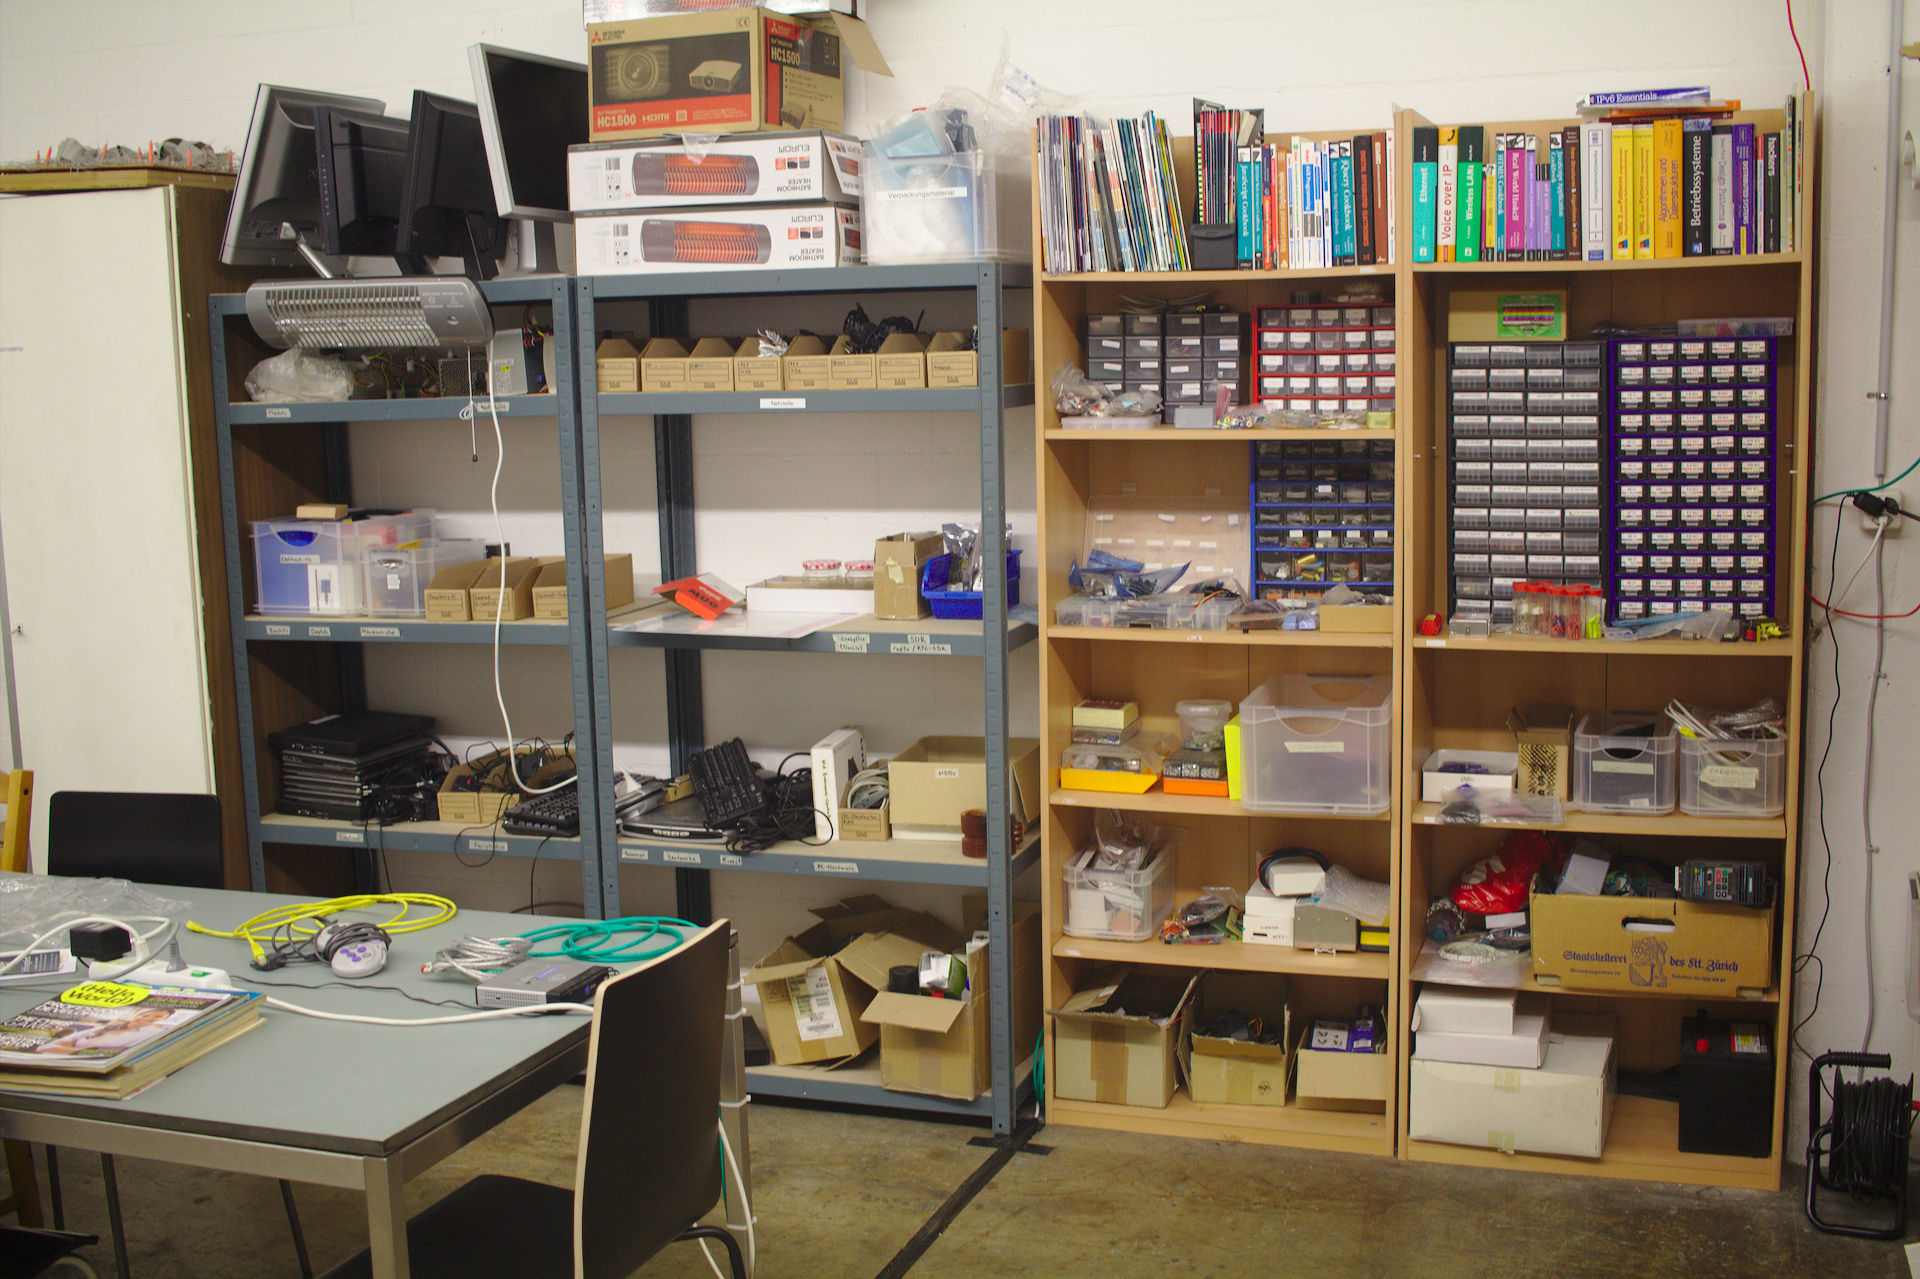
\includegraphics[width=0.5\textwidth]{img/lager.jpg}} & \captionbox*{Messgeräte}{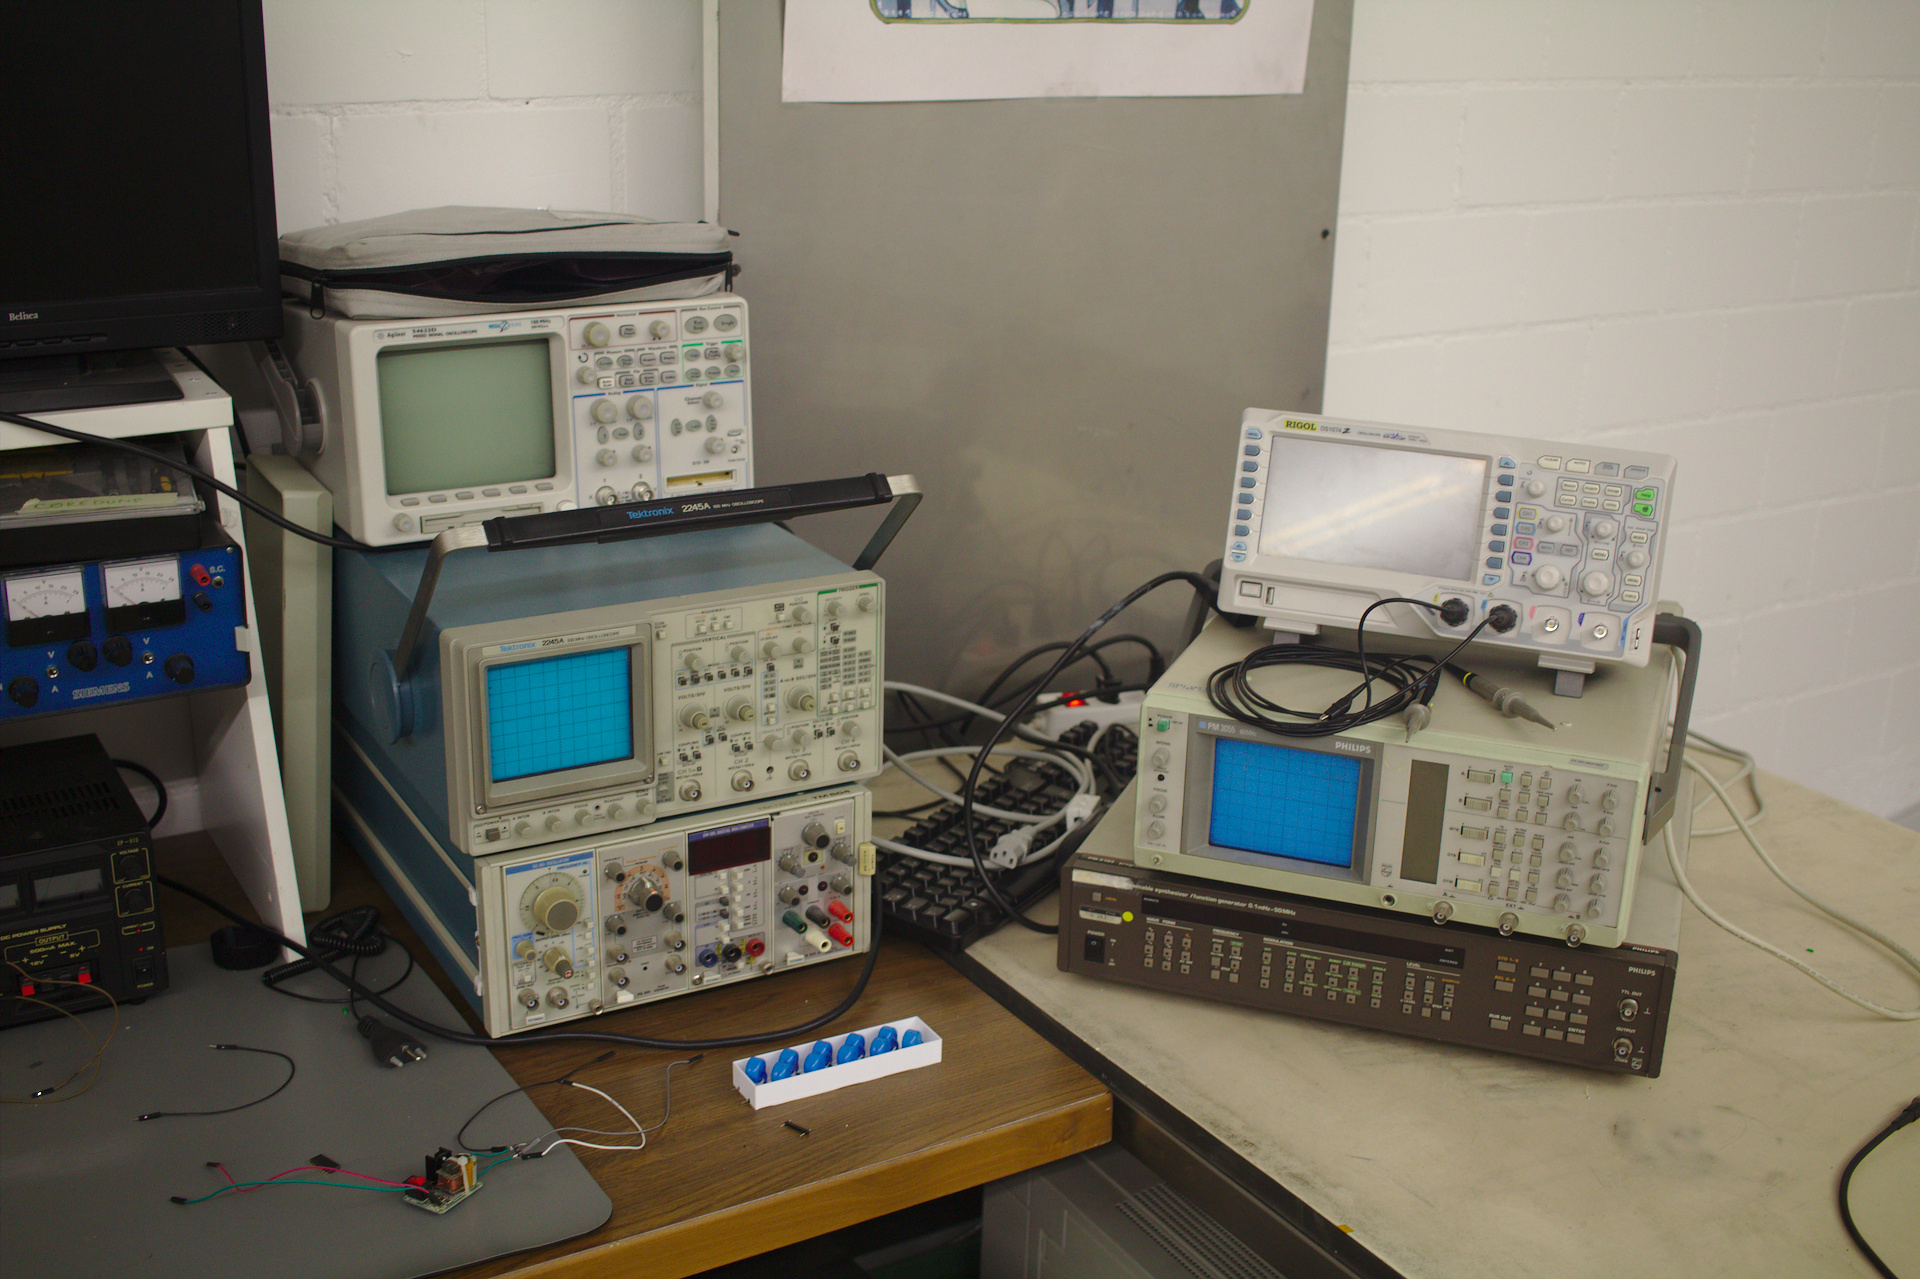
\includegraphics[width=0.5\textwidth]{img/oszis.jpg}} \\
	\captionbox*{Eigene Leiterplatten ätzen}{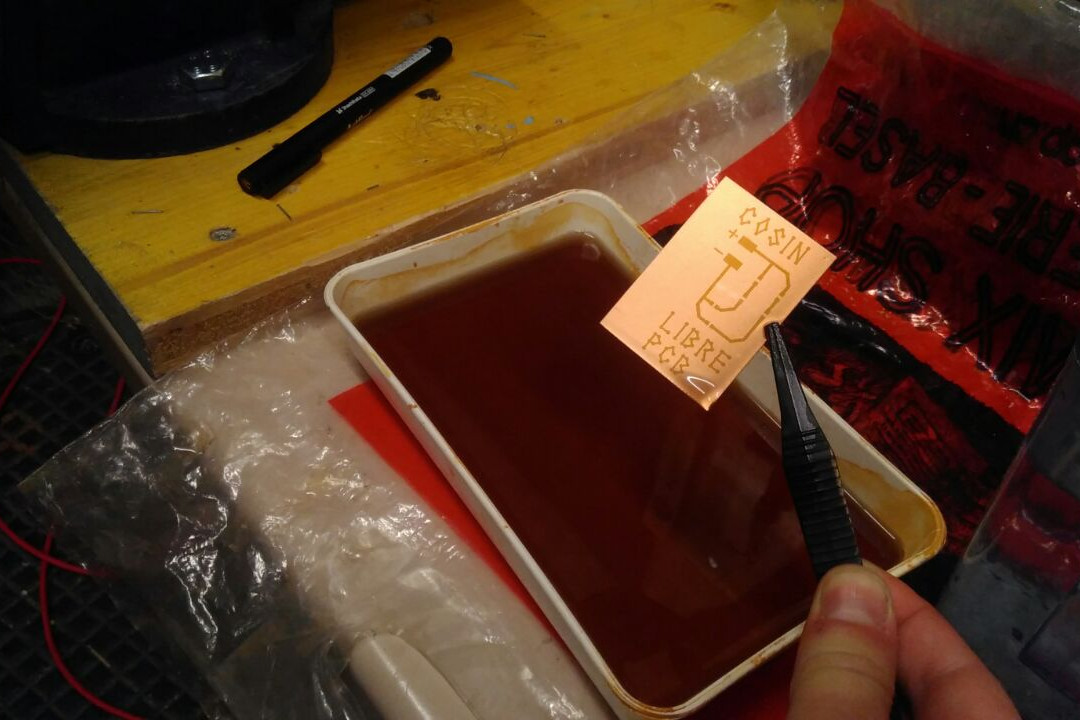
\includegraphics[width=0.5\textwidth]{img/aetzen.jpg}} &
	\captionbox*{Flüssigstickstoff-Glace-Stand am Seenachtfest 2018}{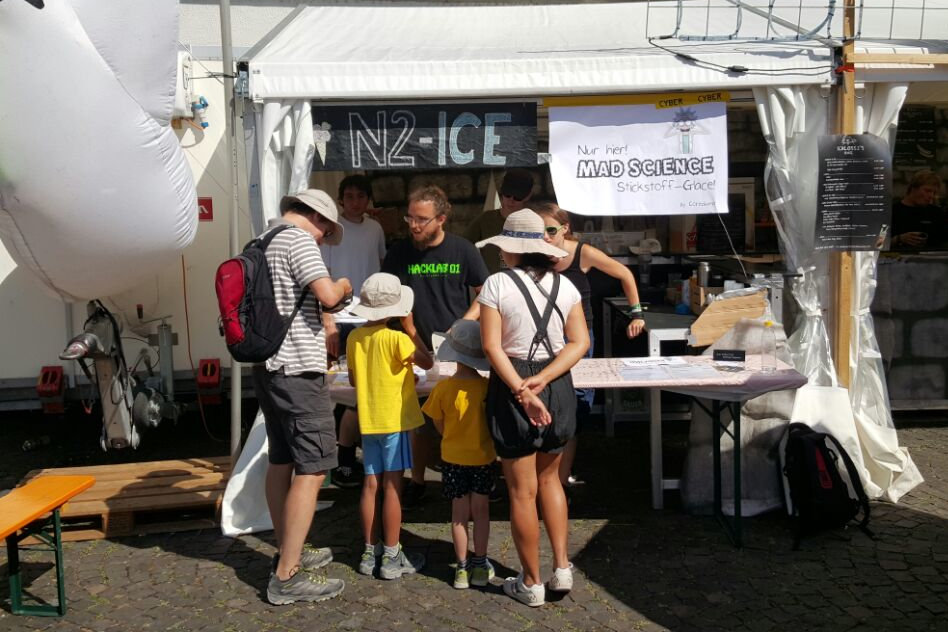
\includegraphics[width=0.5\textwidth]{img/seenachtfest.jpg}} \\
	\captionbox*{Ferienpass 2018: Löten und Programmieren}{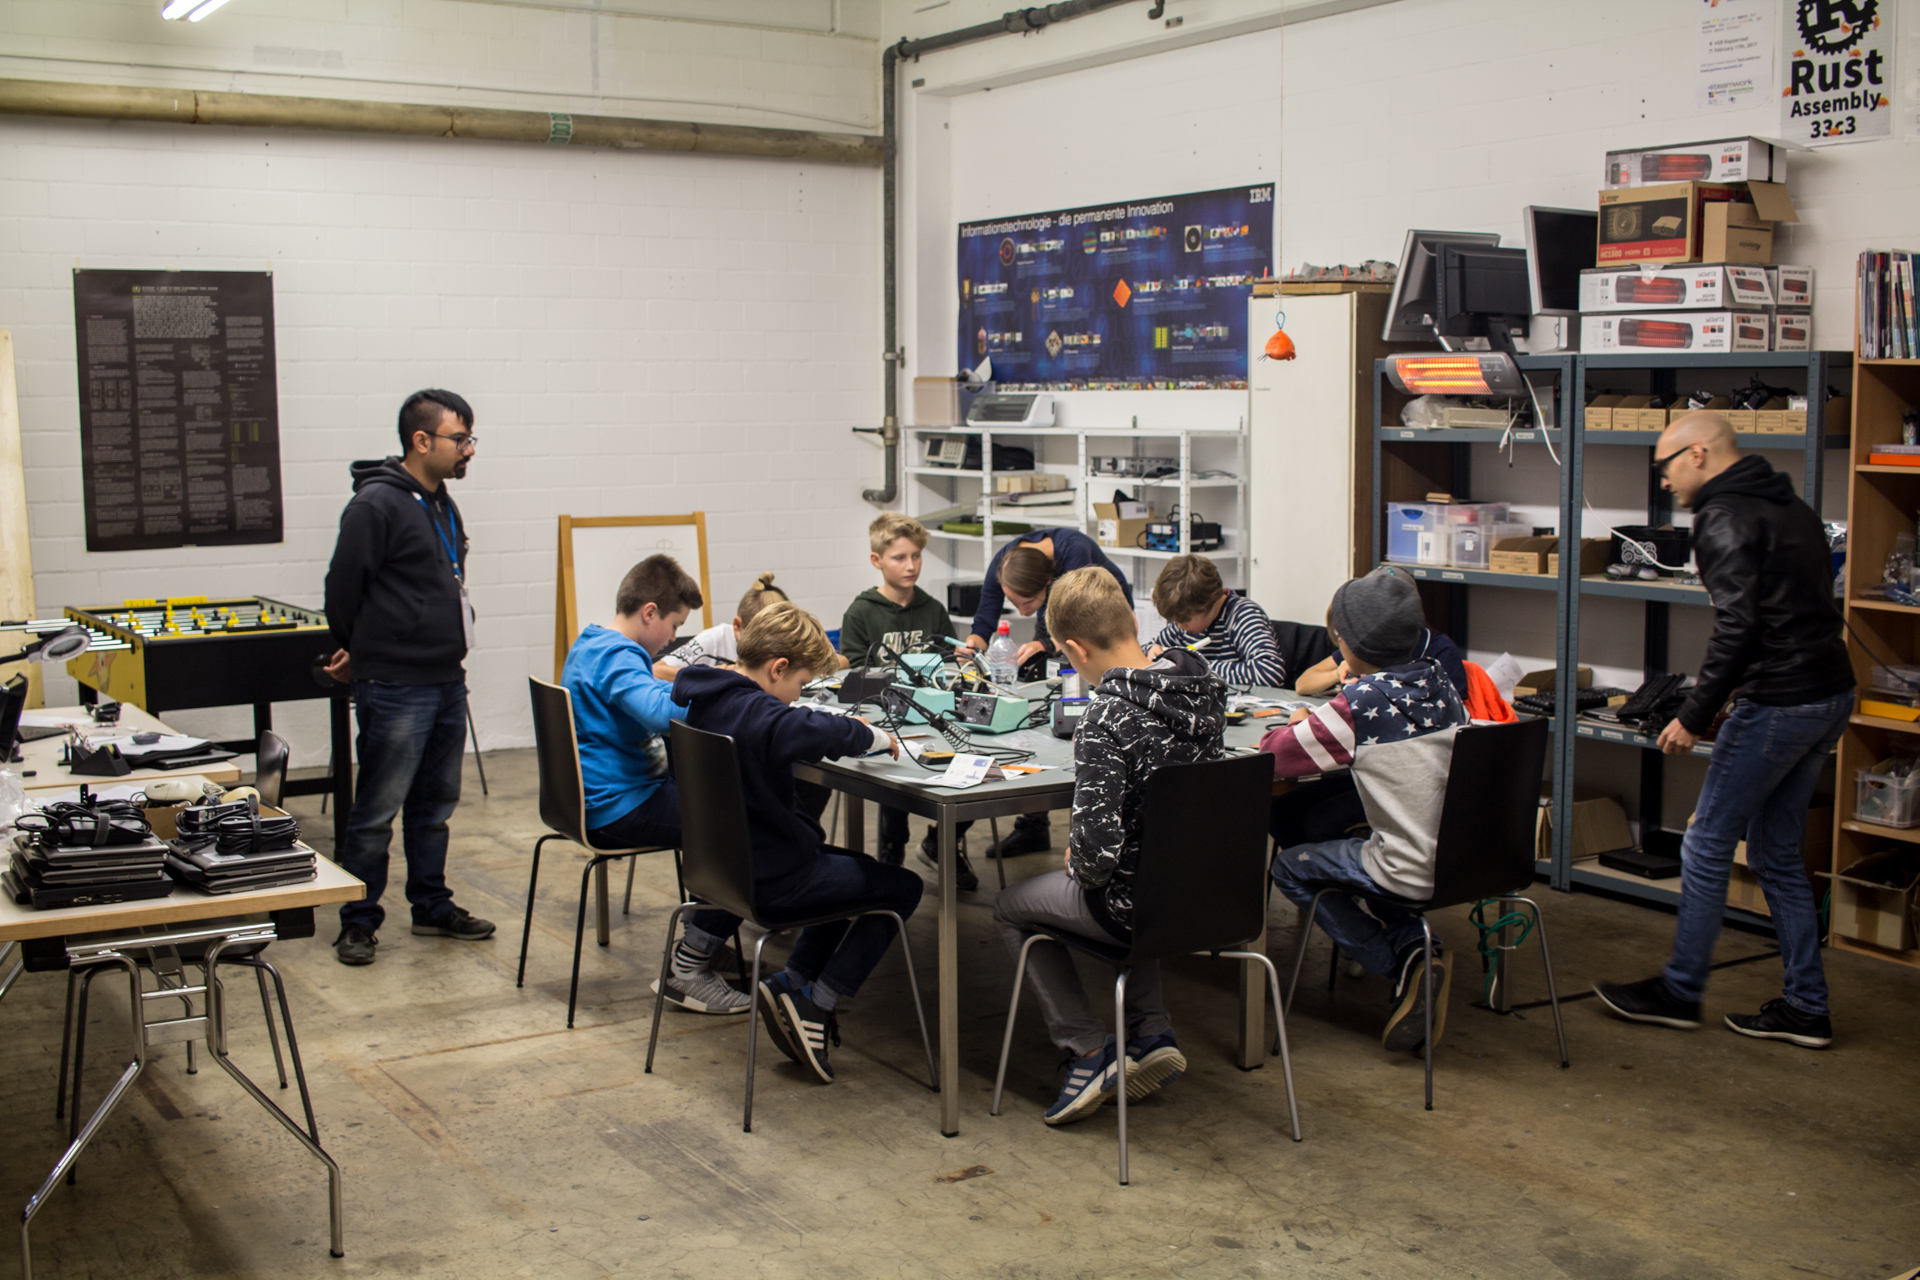
\includegraphics[width=0.5\textwidth]{img/fepa4.jpg}} &
	\captionbox*{Experimente mit Flüssigstickstoff}{\includegraphics[width=0.5\textwidth]{img/n2.jpg}} \\
\end{tabular}
\end{figure}

\end{document}
